\documentclass[a4paper, 12pt, oneside]{article}
\newcommand{\plogo}{\fbox{$\mathcal{PL}$}} 

\usepackage[utf8]{inputenc}
\usepackage[T1]{fontenc} 
\usepackage[spanish]{babel}
\usepackage{fouriernc} 
\usepackage{hyperref}
\usepackage{graphicx}
\usepackage{listings}
%----------------------------------------------------------------------------------------
%	TITLE PAGE
%----------------------------------------------------------------------------------------

\begin{document} 

\begin{titlepage} 

	\centering 
	
	\scshape
	
	\vspace*{\baselineskip} 
	%------------------------------------------------
	%	Title
	%------------------------------------------------
	
	\rule{\textwidth}{1.6pt}\vspace*{-\baselineskip}\vspace*{2pt} 
	\rule{\textwidth}{0.4pt} 
	
	\vspace{0.75\baselineskip} 
	\date{12 Febrero 2018}
	{\LARGE 3.- Paridad binaria  \\} 
	
	\vspace{0.75\baselineskip} 
	
	\rule{\textwidth}{0.4pt}\vspace*{-\baselineskip}\vspace{3.2pt} 
	\rule{\textwidth}{1.6pt} 
	
	\vspace{2\baselineskip} 
	
	%------------------------------------------------
	%	Subtitle
	%------------------------------------------------
	
	Teoría Computacional
	
	\vspace*{3\baselineskip} 
	
	%------------------------------------------------
	%	Editor(s)
	%------------------------------------------------
	
	Por
	
	\vspace{0.5\baselineskip} 
	
	{\scshape\Large García Díaz Ricardo Axel \\} 
    \vspace{2\baselineskip} 
    
    Profesor:  JUAREZ MARTINEZ GENARO 
    
	
	\vspace{15\baselineskip} 
	
	\textit{Escuela Superior de Cómputo \\ Instituto Politécnico Nacional} 
	



\end{titlepage}
\section{Descripción del problema}

El programa evalúa una cadena ingresada o generada por el mismo para verificar su paridad (igual número de 0's y 1's)


\section{Código}
\lstset{language=Python, breaklines=true, basicstyle=\footnotesize}
\begin{lstlisting}[frame=single]
import random
import math
from tkinter import*

archivo = open('datos3.txt','w')

print("Bienvenido al Automata paridad binaria.")
opc = input("Que desea hacer? \n 1)Ingresar cadena. \n 2)Generar cadena\n")

if opc=="1":
	eleccion = input("Ingrese la cadena a evaluar \n")
	palabra = str(eleccion)

else:
	rand = random.randrange(10000)
	palabra = str(bin(rand)[2:])

print ("Cadena a evaluar:",palabra)

c=0 #estado
for x in palabra:

	#estado 0
	if (c == 0 and x == "0"): 
		c = 1
		archivo.write("Se paso del estado q0 al q1 \n")
		continue
	if (c == 0 and x == "1"):
		c = 3
		archivo.write("Se paso del estado q0 al q1 \n")
		continue

	#estado 1
	if (c == 1 and x == "0"):
		c = 0
		archivo.write("Se paso del estado q1 al q0 \n")
		continue
	if (c == 1 and x == "1"): 
		c = 2
		archivo.write("Se paso del estado q1 al q2 \n")
		continue

	#estado 2
	if (c == 2 and x == "1"):
		c = 1
		archivo.write("Se paso del estado q2 al q1 \n")
		continue
	if (c == 2 and x == "0"): 
		c = 3
		archivo.write("Se paso del estado q2 al q3 \n")
		continue

	#estado 3	
	if (c == 3 and x == "0"):
		c = 2
		archivo.write("Se paso del estado q3 al q2 \n")
		continue
	if (c == 3 and x == "1"): 
		c = 0
		archivo.write("Se paso del estado q3 al q0 \n")
		continue
archivo.close

print (c)
if (c == 0):
	print("Se llego al estado final. Se ha generado archivo con historia (datos3.txt) \n La cadena es par")
else:
	print("No se llego al estado final. Se ha generado archivo con historia (datos3.txt) \n La cadena es inpar")

ventana = Tk()
canv = Canvas(ventana,width=400,height=700)
ventana.geometry("400x700")

ventana.title('Automata Paridad')

p= Label(ventana,text="Automata de paridad. \n Cadena:"+palabra).place(x=10,y=10)

#q0
p0= Label(ventana,text="q0").place(x=55,y=105)

if (c==0):
	canv.create_oval(20,70,110,160, fill="green")
else:	
	canv.create_oval(20,70,110,160, fill="blue")
canv.create_oval(35,85,95,145)
canv.create_oval(90,145,100,155, fill="black")
n1= Label(ventana,text="0").place(x=190,y=35)
canv.create_oval(50,155,60,165, fill="black")
n2= Label(ventana,text="0").place(x=190,y=185)

#q1
p1= Label(ventana,text="q1").place(x=305,y=105)

if(c==1):
	canv.create_oval(270,70,360,160, fill="red")
else:
	canv.create_oval(270,70,360,160, fill="blue")
canv.create_oval(280,75,290,85, fill="black")
n3= Label(ventana,text="1").place(x=255,y=230)
canv.create_oval(300,155,310,165, fill="black")
n4= Label(ventana,text="1").place(x=360,y=230)

#e2
p2= Label(ventana,text="q2").place(x=305,y=355)

if(c==2):
	canv.create_oval(270,320,360,410, fill="red")
else:
	canv.create_oval(270,320,360,410, fill="blue")
canv.create_oval(280,325,290,335, fill="black")
n5= Label(ventana,text="0").place(x=190,y=285)
canv.create_oval(320,315,330,325, fill="black")
n6= Label(ventana,text="0").place(x=190,y=435)

#e3
p3= Label(ventana,text="q3").place(x=55,y=355)
if(c==3):	
	canv.create_oval(20,320,110,410, fill="red")
else:	
	canv.create_oval(20,320,110,410, fill="blue")
canv.create_oval(90,395,100,405, fill="black")
n7= Label(ventana,text="1").place(x=10,y=230)
canv.create_oval(70,315,80,325, fill="black")
n8= Label(ventana,text="1").place(x=110,y=230)

#lineas
#0-1
xy1 = 95, 60, 286, 105
canv.create_arc(xy1, start=0, extent=180, style="arc")
#1-0
xy2 = 95, 180, 286, 115
canv.create_arc(xy2, start=0, extent=-180, style="arc")

#1-2
xy3 = 286, 160, 356, 320
canv.create_arc(xy3, start=-90, extent=180, style="arc")
#2-1
xy4 = 276, 160, 336, 320
canv.create_arc(xy4, start=90, extent=180, style="arc")

#2-3
xy5 = 95, 430, 286, 365
canv.create_arc(xy5, start=0, extent=-180, style="arc")
#3-2
xy6 = 95, 310, 286, 355
canv.create_arc(xy6, start=0, extent=180, style="arc")

#3-1
xy7 = 36, 160, 106, 320
canv.create_arc(xy7, start=-90, extent=180, style="arc")
#1-3
xy8 = 26, 160, 96, 320
canv.create_arc(xy8, start=90, extent=180, style="arc")

if(c==0):
	p= Label(ventana,text="La cadena es par").place(x=10,y=460)
else:
	ip= Label(ventana,text="La cadena es inpar").place(x=10,y=460)

canv.place(x=0,y=0)
ventana.mainloop()
\end{lstlisting}

\section{Capturas}

Prueba manual
 
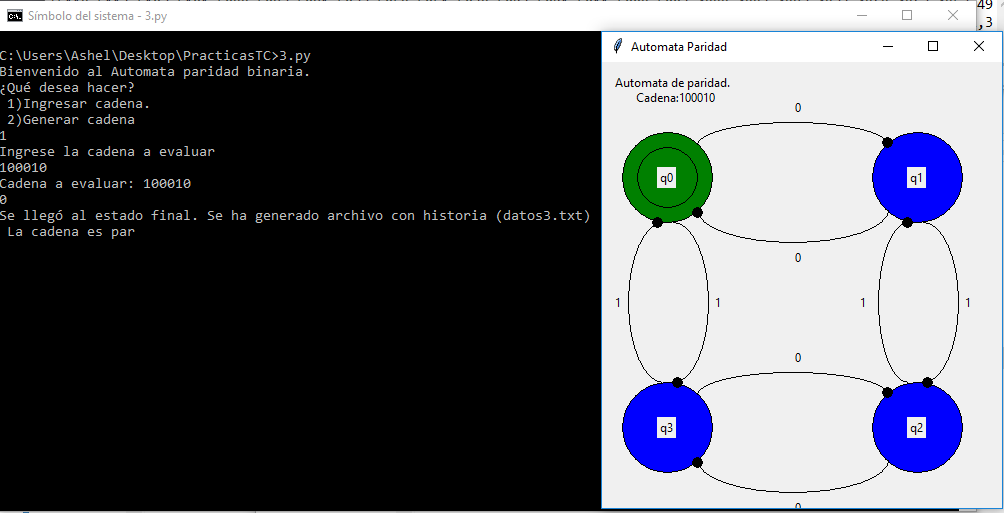
\includegraphics[width=1.2\textwidth]{30.PNG}\\
\\
\clearpage
(documento de texto generado)\\
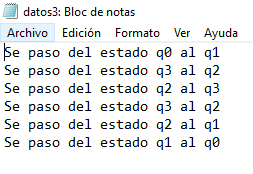
\includegraphics{31.PNG}
\\\\
Prueba automática\\
 
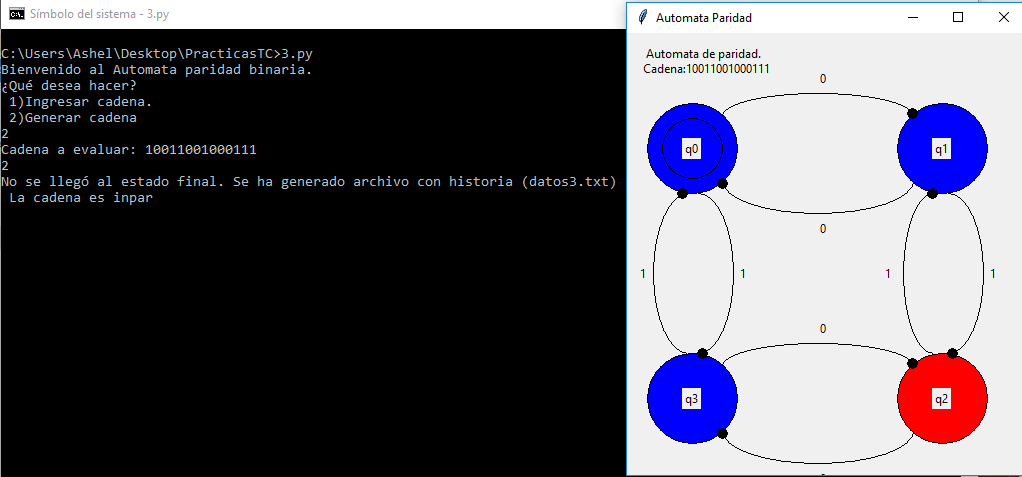
\includegraphics[width=1.2\textwidth]{32.PNG}\\
\\\clearpage
(documento de texto generado)\\
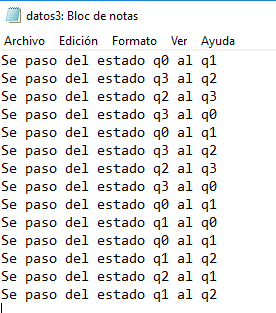
\includegraphics{33.PNG}

\end{document}

\end{document}

%----------------------------------------------------------------------------------------

\end{document}
